% !TEX options=--shell-escape
\documentclass[usenames,dvipsnames,9pt]{beamer}

\makeatletter
\def\input@path{{../support/beamer-template/}}
\makeatother

\usepackage{../support/beamer-template/beamerthememetropolis}

\usepackage[utf8]{inputenc}
\usepackage[czech]{babel}
\selectlanguage{czech}

\usepackage{hyperref}
\usepackage{fontawesome}
\usepackage{minted}
\usepackage{mathtools}
\usepackage{tabularx}
\usepackage{smartdiagram}
\usepackage{amssymb}
\usepackage{qrcode}

% Commands shared between most of the tutorial slides

% Homework deadlines
\newcommand{\hwVIIdeadline}{10. 5. 2020}



% Download icon and text with link relative to the root of the courseware site
\newcommand{\download}[1]{\hfill\faDownload\hspace{5pt}\href{https://cw.fel.cvut.cz/wiki/_media/courses/be4m36mas/#1}{\tt #1}\\[1.3em]}

% Draw eye icon
\newcommand{\see}[1]{\faEye\hspace{5pt}#1}

\newcommand{\sep}{\hspace{10pt}/\hspace{10pt}}

\def\Ipe#1{\def\IPEfile{#1}\input{#1}}

% Draw pacman icon
\newcommand{\pacman}[1]{\tikz[baseline=.1em,scale=.6]{
    \useasboundingbox (.02,0) rectangle (.6,.6);
  \draw [fill=#1] (.3,.3) -- ++(25:.3) arc (+25:+335:.3) -- cycle;

}}

% Draw ghost icon
\newcommand{\ghost}[1]{\tikz[baseline=.1em,scale=.5]{
  \draw [fill=#1] (0,0) -- (0,.5) arc (+180:0:.3) -- (.6,0) --
  (.5,.15) -- (.4,0) -- (.3,.15) -- (.2,0) -- (.1,.15) -- cycle;
    \coordinate (eye) at (360*rand:.03);
    \foreach \x in {.17,.43}{
      \fill[white] (\x,.5) circle[radius=.1];
      \fill[black] (\x,.5) ++(eye) circle[radius=.05];
    }
}}

\newcommand{\desc}[2]{
  #1

  \vspace{-0.6em}
  \hfill\begin{minipage}{0.9\linewidth}
    #2
  \end{minipage}

  \vspace{0.2em}
}

\newcommand{\redc}{\tikz\draw[red,fill=red] (0,0) circle (.5ex);}

\newcommand{\greenc}{\tikz\draw[green,fill=green] (0,0) circle (.5ex);}


% Default url for generating QR code with feedback form.
\newcommand{\defaultfeedbackurl}{https://forms.gle/vwbWazEu14w1Kf487}

% Generate frame with QR code to a feedback form.
\newcommand{\framefeedback}[1][\defaultfeedbackurl]{
  \begin{frame}[standout]
    \begin{minipage}{0.4\linewidth}
      \begin{center}
        \textbf{\LARGE Díky za pozornost!}
      \end{center}

      \vspace{3em}

      \raggedleft\small Budeme rádi za Vaši\\zpětnou vazbu! $\rightarrow$
    \end{minipage}
    \hfill
    \begin{minipage}{0.5\linewidth}
      \vspace{4em}
      \centering\qrcode[height=\linewidth]{#1}\\
      \vspace{0.8em}
      \url{#1}
    \end{minipage}
  \end{frame}
}

\title{Konkurentní datové struktury}
\date{}
\institute{B4B36PDV -- Paralelní a distribuované výpočty}

\metroset{block=fill}

\begin{document}
\maketitle

%\begin{frame}
%  Minulé cvičení:
%  \begin{center}
%    \Large\emph{``Paralelní programování v OpenMP...''}
%  \end{center}
%  \pause
%  \vspace{1.5em}
%  
%  Zajištění konzistentního přístupu do paměti pro více vláken je složité a pomalé. Jak navrhnout strukturu ukládání dat tak, aby operace byly rychlé a mohlo s ní pracovat více vláken součastně?
%
%  \pause
%  \vspace{2.5em}
%  Dnešní menu: \hspace{10pt} \huge Konkurentní datové struktury
%\end{frame}

\begin{frame}[t]
  Minulé cvičení:
  \begin{center}
    \Large\emph{``Paralelní programování v OpenMP...''}
  \end{center}
  
 % \pause

\begin{figure}
  \only<2>{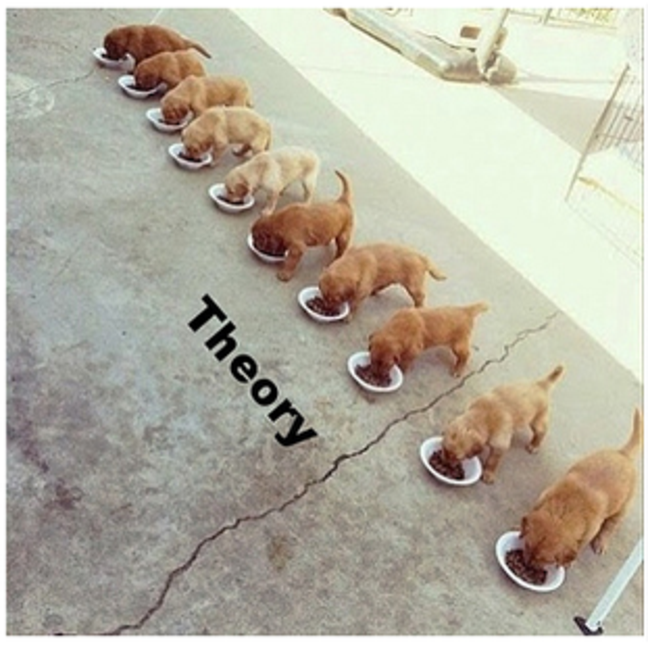
\includegraphics[scale=0.4]{figs/theory.pdf}}%
  \only<3->{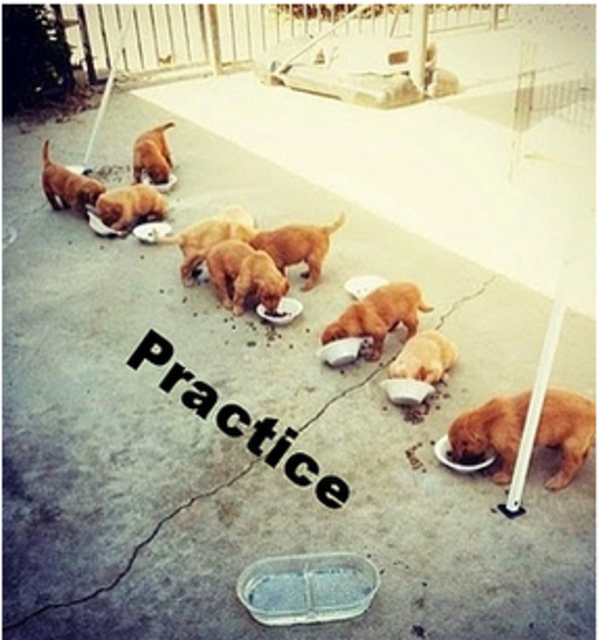
\includegraphics[scale=.4]{figs/practice.pdf}}%
\end{figure}

%\pause

  \only<4>{Dnešní menu: \hspace{10pt} \huge Konkurentní datové struktury}
\end{frame}

\begin{frame}
  \frametitle{Osnova}
  \begin{itemize}
    \item Opakování z minulého cvičení
    \item Zámková architektura datových struktur
    \item Bezzámková architektura datových struktur\\[1.5em]
    \item Zadání třetí domácí úlohy
  \end{itemize}
\end{frame}

\section{Opakování z minulého cvičení}
\begin{frame}[standout]
  \Huge
  \url{http://goo.gl/a6BEMb}
\end{frame}


\begin{frame}[fragile]
  \frametitle{Co provádí následující kód? Co bude po skončení v data?}

\begin{minted}{c}
unsigned int num_threads = omp_get_num_threads();
unsigned int thread_id = omp_get_thread_num();
std::vector<int> data(100000);
#pragma omp parallel
{
	int chunk_size = 1 + data.size() / num_threads;
	int begin = thread_id * chunk_size;
	int end = std::min ( data.size(), 
		(thread_id + 1) * chunk_size );
	for (unsigned int i = begin; i < end; i++)
		data[i] ++ ;
}
\end{minted}
  
\vspace{2em}
  
  {\bf Napište odpověď}

\end{frame}

\begin{frame}[fragile]
  \frametitle{Jakým způsobem bude následující kód proveden?}

\begin{minted}{c}
std::vector<int> data(100000);
int size = data.size();
#pragma omp parallel
{
	#pragma omp parallel for
	for (unsigned int i = 0; i < size; i++)
		data[i] ++ ;
}
\end{minted}
  
  \vspace{2em}
  
  {\bf Zvolte co se může stát}
  
  \begin{enumerate}
  \item Kód nelze zkompilovat
   \item OpenMP rozdělí práci na for cyklu mezi dostupná fyzická vlákna
    \item Vnitřní smyčka bude provedena serielně
     \item OpenMP vytvoří více vláken než fyzicky lze a dojde k degradaci výkonu
     \item For smyčka bude provedena každým vláknem celá
  \end{enumerate}

\end{frame}

\begin{frame}[fragile]
  \frametitle{K čemu dojde u následujícího kódu?}

\begin{minted}{c}
int k = 0;
std::vector<int> data = getRandomVectorOfSize(400);
#pragma omp parallel num_threads(4)
{
	int begin = omp_get_thread_num() * 100;
	int end = (1 + omp_get_thread_num()) * 100;
	for (unsigned int i = begin; i < end; i++)
		#pragma omp critical
		k += data[i];
}
\end{minted}
  
  \vspace{2em}
  
  {\bf Zvolte co se může stát}
  
  \begin{enumerate}
  \item Dojde k efektivní paralelizaci výpočtu
  \item OpenMP zvládne distribuovat sčítání mezi vlákny aby nedošlo k degradaci výkonu
  \item OpenMP bude zbytečně často serializovat vlákna pomocí critical
  \item OpenMP bude naprosto zbytečně serializovat vlákna pomocí critical
  \end{enumerate}

\end{frame}

\section{Tvorba konkurentních datových struktur}

\begin{frame}
\frametitle{Co bychom si přáli?}

Aby jednu strukturu používalo více vláken {\bf současně}.

  \begin{center}
    \Large Co musíme změnit oproti frontě z prvního domácího úkolu?
  \end{center}
  
\pause\vspace{1em}\hrule\vspace{1em}

\begin{itemize}
  \item Nesmíme zamykat \textbf{celou} datovou strukturu!
  \item Se zamykáním zámků musíme šetřit
\end{itemize}

\vspace{1em}\hfill\faWarning \hspace{2pt} Jinak se datová struktura stane brzdou výpočtu!

\end{frame}

\begin{frame}
  Možný přístup:
  \begin{enumerate}
    \item Vezmu kód existující jednovláknové datové struktury
    \item Ve chvíli, kdy strukturu dělám nějaké zásahy, zamknu si část struktury pro sebe
  \end{enumerate}
  \begin{center}
    \Large Je to opravdu takto lehké?
  \end{center}
  \pause\vspace{1em}\hrule\vspace{1em}
  Typický vzor práce s jednovláknovými strukturami:
  \begin{center}
    Příprava $\rightarrow$ ``Poškození'' dat $\xrightarrow{\text{\textcolor{red}{\faFlash}}}$ Oprava $\rightarrow$ Hotovo!
  \end{center}

  \pause\vspace{1em}
  Musíme zabránit použití ``rozbité'' části = vyloučit i čtenáře\\
  (a zamykat si části struktury, i když to není potřeba -- např. při čtení)

  \pause\vspace{1.5em}

  \hfill \large\bf To si ale moc nepomůžeme :-(
\end{frame}

\begin{frame}
  \frametitle{Jak to tedy udělat lépe?}
  \begin{enumerate}
    \item \Large Strčit hlavu do písku a (téměř) nezamykat
    \item \Large Když nastane problém, tak ho (nějak) vyřešit
  \end{enumerate}
  \hfill To se snáz řekne, než udělá...

  \pause\vspace{1em}\hrule\vspace{1em}
  Některé z možných problémů:
  \begin{itemize}
    \item \textbf{Datová struktura se může nacházet v mezistavu:}\\
          Buď musí být použitelná, nebo si musíme být jistí, že problém detekujeme, než poškodíme data
    \item \textbf{Nesmíme uvolnit paměť, pokud s ní pracuje jiné vlákno:}\\
          Složitější datové struktury často využívají techniky podobné garbage-collectoru v Javě.
  \end{itemize}
\end{frame}

\begin{frame}
  \frametitle{Jak to tedy udělat lépe?}
  O takových datových strukturách se těžko přemýšlí...

  \hfill ... a ještě hůř se v nich hledají chyby!

  \vspace{2em}

  \small\see{\url{http://libcds.sourceforge.net}}

  \see{C++ Concurrency In Action: Practical Multithreading}
\end{frame}

% \section{Zámková architektura datových struktur}

% \begin{frame}

% Místo zamykání celé struktury zamykáme {\bf části} struktury

% \faWarning \hspace{3pt} Uvolňujeme zámky co nejdříve!

% \vspace{2em}

% Vhodné je použití \textit{spinlocků} = systémový busy waiting po velmi krátkou dobu.
%      \begin{itemize}
%     \item[\ \ \ \ \ $\rightarrow$] Efektivnější než řešit synchronizaci
%     \item[\ \ \ \ \ $\rightarrow$] Paměťově nenáročné (2.5\% oproti mutexu v Linuxu)
%   \end{itemize}

% \end{frame}

\section{Cvičení: konkuretní spojový seznam}

{\setbeamertemplate{frame footer}{\see{{\tt lockBased.cpp}, {\tt main.cpp} \sep {\tt make main}}}
\begin{frame}[fragile]
  \frametitle{Konkurentní spojový seznam}
  
  Reprezentace seznamu prvků
  \begin{itemize}
    \item My ho budeme chtít mít seřazený vzestupně...
    \item Vložení prvku = nalezení správné pozice + vložení nového uzlu
  \end{itemize}  
  
  \vspace{1em}

  \begin{figure}
    \centering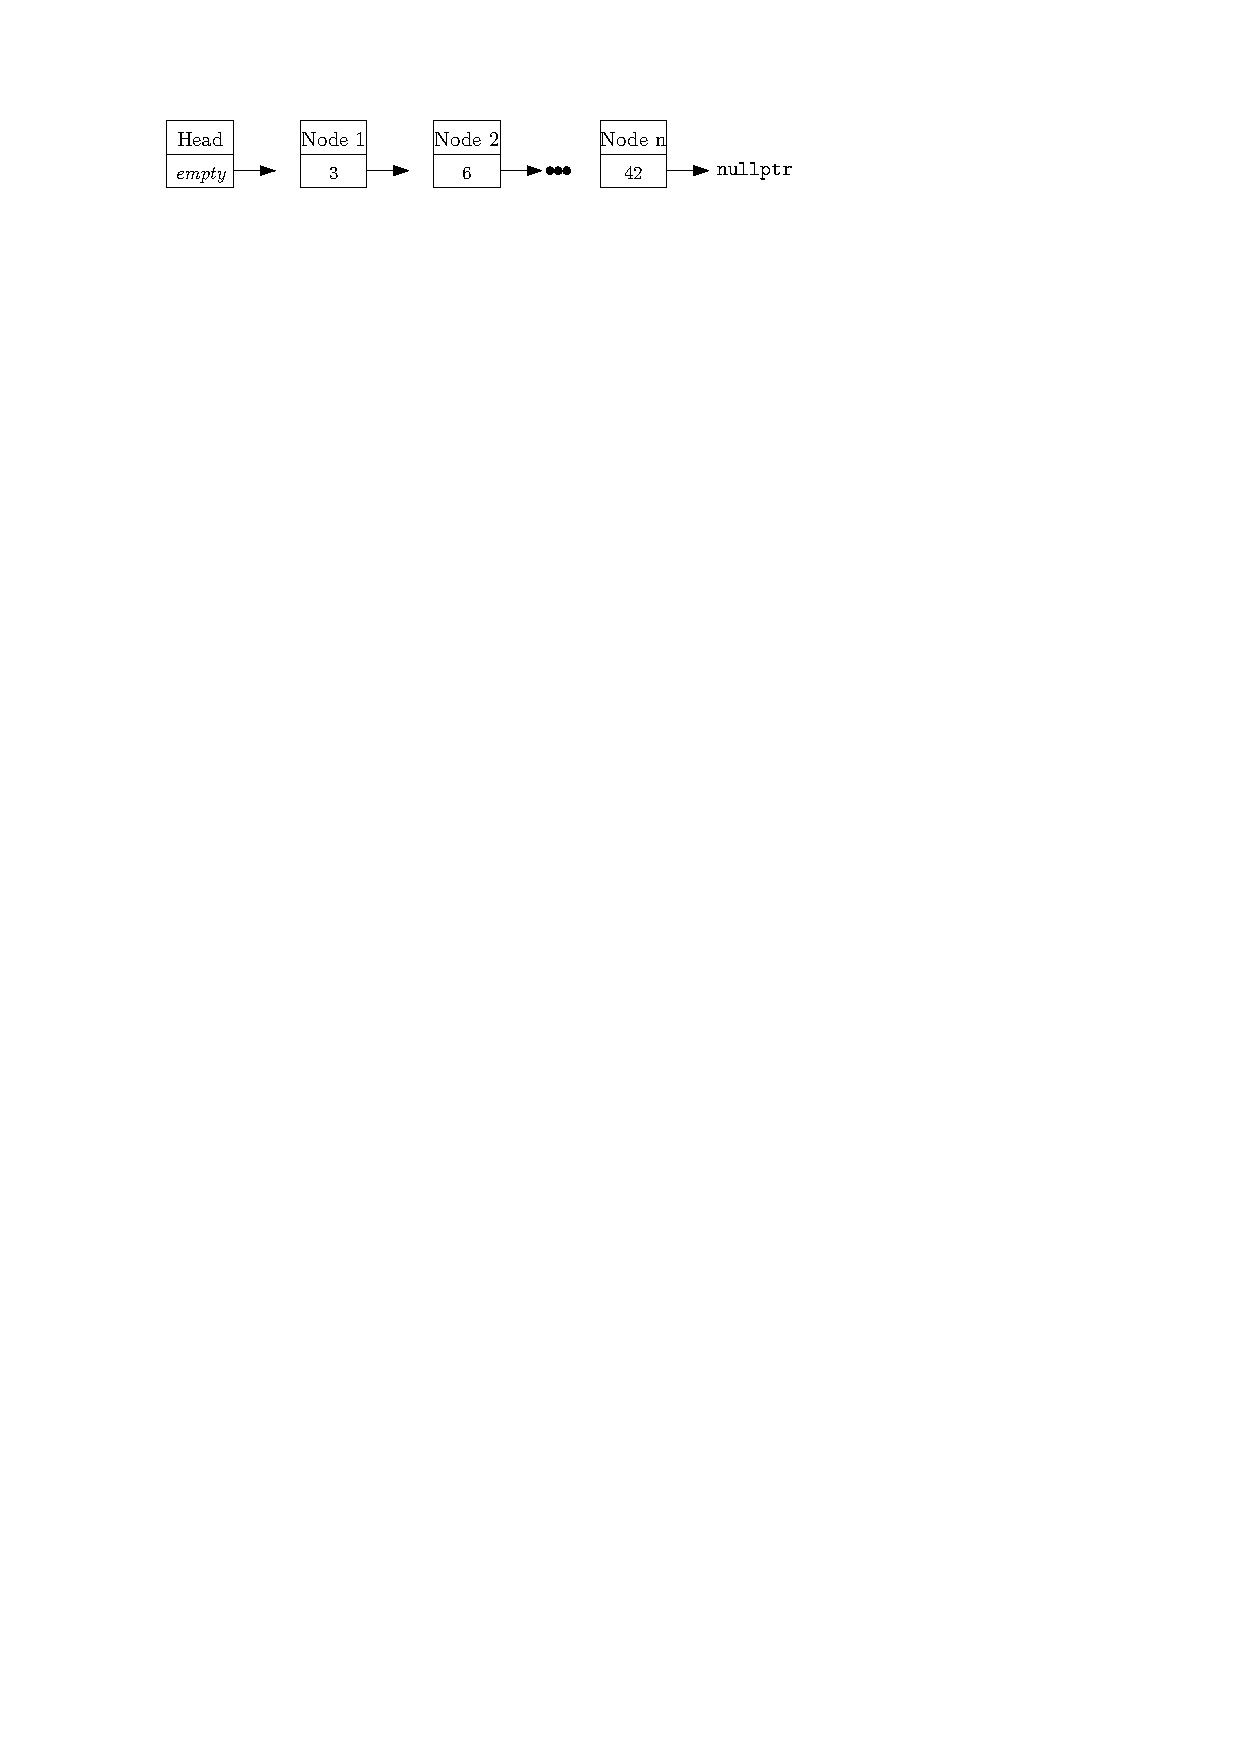
\includegraphics{figs/linkedList.pdf}
  \end{figure}
  
    \pause

  \vspace{2em}
  
  \begin{block}{Doimplementujte metodu \texttt{insert}}
    Doimplementujte tělo metody \texttt{insert} v souboru \texttt{lockBased.h}.
    Pro synchronizaci vláken použijte \texttt{spin\_lock} (používá se stejně jako \texttt{std::mutex}), který umístíte ke každému uzlu seznamu.
    Snažte se zámky zamykat pouze na čas modifikace seznamu a pouze tam, kde jsou potřeba!
  \end{block}
\end{frame}
}

\begin{frame}[fragile]
  \frametitle{Data race}

  Nesynchronizované přístupy do paměti (s alespoň jedním zápisem) jsou ve standardu C++ vedené jako
  \begin{center}
    \Large \faWarning \hspace{3pt} \emph{undefined behavior} \hspace{1pt} \faWarning
  \end{center}

  Může se nám stát spousta špatných věcí, například:\\
  (ty navíc závisí na kompilátoru a platformě)
  \begin{itemize}
    \item Můžeme přečíst částečně zapsaná data (\emph{dirty read})
    \item Vlákno se nedozví o změně provedené jiným vláknem
    \item Vlákno se dozví pouze o části provedených změn
  \end{itemize}

  \pause\vspace{2em}
  \begin{center}
    {\Large \texttt{std::atomic}} \\
    Synchronizace přístupů ke stejné proměnné zajištěna
  \end{center}
\end{frame}

\begin{frame}
  \begin{center}
    \Large Můžeme se zámků zbavit úplně?
  \end{center}
\end{frame}

\section{Bezzámková architektura datových struktur}

\begin{frame}

  Navrhnout správně zamykání je náročné

  \begin{itemize}
    \item Špatné použití může vést k deadlocku
    \item Velké množství zámků snižuje potenciál opravdové konkurence 
    \item Paměťový overhead (\texttt{std::mutex} na Linuxu má 40B!)
  \end{itemize}
  
  \pause
  \begin{center}
    \Large Jak na to?
  \end{center}

  \pause
 
  \begin{itemize}
  \item[\ \ \ \ \ $\rightarrow$] Pomocí atomických operací s pamětí
  \end{itemize}

\end{frame}

\begin{frame}[fragile]
  \frametitle{Porovnej a prohoď}
  \textbf{Klíčová} operace pro \emph{lock-free} datové struktury.
  \vspace{2em}

  Porovnej a prohoď (neboli \textit{compare-and-swap}) je atomická operace s pamětí na objektu \texttt{std::atomic<T> X}, definovaná v C++ jako 

  \begin{minted}{c}
  bool X.compare_exchange_strong( T& expected, T desired)
  \end{minted}
  
  která ma funkcionalitu ekvivalentní 
  
  \begin{minted}{c}
  if ( X == expected ){ X = desired; return true; }
  else{ expected = X; return false; }
  \end{minted}
  
  \pause\vspace{1em}
  
  Kontrolu a změnu datové struktury lze provést {\bf atomicky}!

\end{frame}

{\setbeamertemplate{frame footer}{\see{{\tt lockFree.cpp}, {\tt main.cpp} \sep {\tt make main}}}
\begin{frame}[fragile]
  \begin{block}{Doimplementujte metodu \texttt{insert}}
    Doimplementujte tělo metody \texttt{insert} v souboru \texttt{lockFree.h}.
    Namísto použití zámků nyní použijte atomickou operaci \emph{compare-and-swap} pro úpravu pointerů ve spojovém seznamu.
  \end{block}

  \vspace{2em}\hrule\vspace{2em}
  \pause
  \textbf{Bonusové úlohy:}
  \begin{enumerate}
    \item Zkuste se zamyslet, zda byste dokázali naimplementovat i dvousměrný spojový seznam
    \item Zkuste naimplementovat spojový seznam, ve kterém může kromě přidávání docházet konkurentně i k mazání prvků
  \end{enumerate}
\end{frame}
}


\section{Zadání třetí domácí úlohy}

\begin{frame}[fragile]
  \frametitle{Konkurentní binární vyhledávací strom}
  
    \begin{minipage}{0.6\linewidth}
    Struktura, v níž jsou jednotlivé prvky uspořádány tak, aby bylo možné rychle vyhledávat
    \vspace{2em}
    \begin{itemize}
    \item každý uzel tedy má nanejvýš dva potomky;
    \item každému uzlu je přiřazen určitý klíč;
    \item levý podstrom uzlu obsahuje klíče menší než je klíč uzlu; a
    \item pravý podstrom uzlu obsahuje klíče větší než je klíč uzlu.
    \end{itemize}
  \end{minipage}
  \hfill
  \begin{minipage}{0.3\linewidth}
    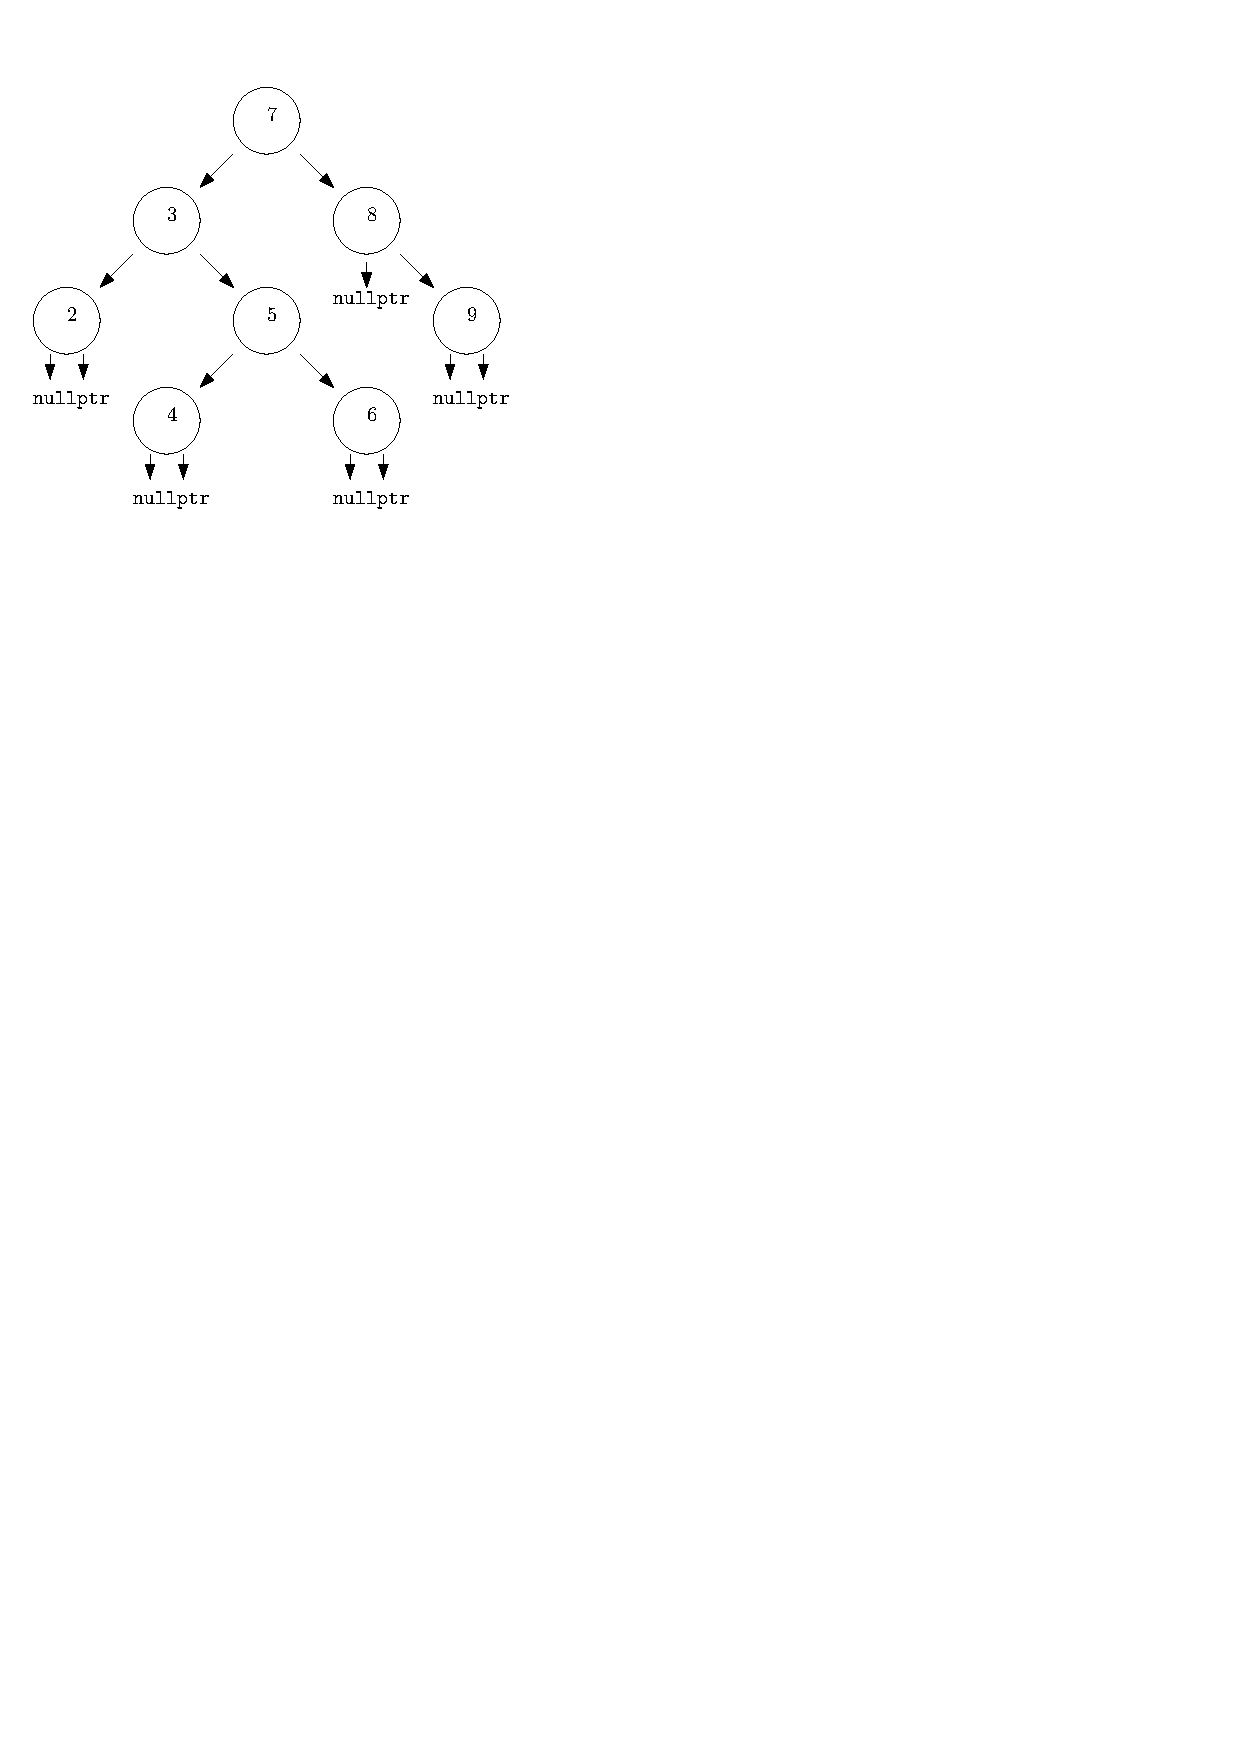
\includegraphics[width=1.3\linewidth]{figs/bst.pdf}
  \end{minipage}
\end{frame}

\begin{frame}
  \frametitle{Konkurentní binární vyhledávací strom}
  Naimplementujte metody v \texttt{bst\_tree.cpp} a \texttt{bst\_tree.h} a zajistěte, že
  \begin{enumerate}
    \item každý prvek je vložet právě jednou; a
    \item žádný vložený prvek se neztratí.
  \end{enumerate}
  
  Zpracování musí být {\bf konkurentní}, nikoli serielní!
  
  \pause\vspace{1.5em}
  
  Za spravné výsledky a vysoký stupeň konkurence dostanete až {\bf 2b}.
  
    \pause\vspace{1.5em}

Soubory \texttt{bst\_tree.cpp} a \texttt{bst\_tree.h} nahrajte do systému BRUTE.
  

\end{frame}


% Frame with the feedback QR code 
\framefeedback{}



\end{document}
